%%%%%%%%%%%%%%%%%%%%%%%%%%%%%%%%%%%%%%%%%%%%%%%%%%%%%%%%
\begin{figure*}[t]
    \centering
    \begin{subfigure}{0.3\textwidth}
        \centering
        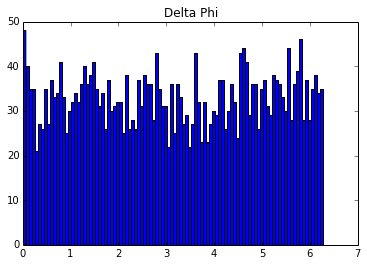
\includegraphics[width=\textwidth]{images/deltaphi}
        \subcaption{}
        \label{subfig:robust-deltaphi}
    \end{subfigure}
    \;
    \begin{subfigure}{0.3\textwidth}
        \centering
        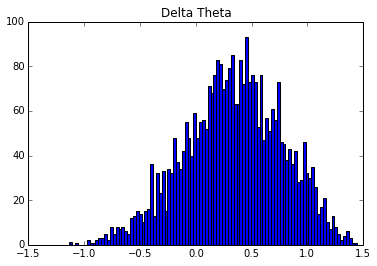
\includegraphics[width=\textwidth]{images/deltatheta}
        \subcaption{}
        \label{subfig:robust-deltatheta}
    \end{subfigure}
    \;
    \begin{subfigure}{0.3\textwidth}
        \centering
        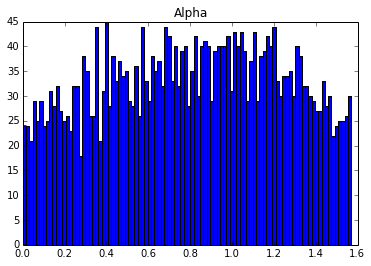
\includegraphics[width=\textwidth]{images/alpha}
        \subcaption{}
        \label{subfig:robust-alpha}
    \end{subfigure}
    \caption{Empirical results on the robustness of the proposed cosine of normals. (a) $\Delta \phi$ distribution (b) $\Delta \theta$ distribution (c) $\alpha$ distribution.}
    \label{fig:robust-properties}
\end{figure*}
%%%%%%%%%%%%%%%%%%%%%%%%%%%%%%%%%%%%%%%%%%%%%%%%%%%%%%%%
%%%%%%%%%%%%%%%%%%%%%%%%%%%%%%%%%%%%%%%%%%%%%%%%%%%%%%%%
\section{Properties of Normals}\label{sec:properties-of-normals}
%%%%%%%%%%%%%%%%%%%%%%%%%%%%%%%%%%%%%%%%%%%%%%%%%%%%%%%%
\begin{figure}[t]
    \centering
    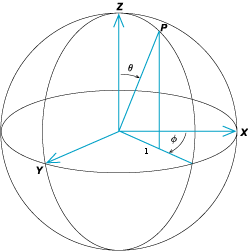
\includegraphics[width=0.6\columnwidth]{images/spherical-coordinates}
    \caption{The spherical coordinate system assumed in this paper.}
    \label{fig:spherical-coordinates}
\end{figure}
%%%%%%%%%%%%%%%%%%%%%%%%%%%%
It is important to clarify the properties of the subspace of normals, before attempting any statistical analysis on them. In particular, there are a number of ways in which we can parametrise normals at a given point. The simplest way to denote a normal is as a 3-component unit vector, $\boldsymbol{n} = [x, y, z]^T$. However, as is commonly noted in SFS literature, normals are uniquely defined by just two parameters. In SFS literature, these parameters are $p$ and $q$ and are related to the normal by the following relationship:
%%%%%%%%%%%%%%%%%%%%%%%%%%%%
\begin{equation}\label{eq:pq-representation}
    \boldsymbol{n} = \frac{[p, q, -1]^T}{\sqrt{p^2 + q^2 + (-1)^2}}
\end{equation}
%%%%%%%%%%%%%%%%%%%%%%%%%%%%
Here, $p$ and $q$ represent the local surface gradients $\left( \frac{\partial z}{\partial x}, \frac{\partial z}{\partial y} \right)$. However, as noted by Smith and Hancock in \cite{RefWorks:90}, a more useful depiction of normals is as points that lie on the surface of a unit sphere. Since each normal lies on this surface, we can uniquely define a given normal in terms of it's spherical coordinates, azimuth ($\phi$) and elevation ($\theta$), which is illustrated in Figure~\ref{fig:spherical-coordinates}. The azimuth angle represents rotation within the $xy$-plane and has range $[0, 2 \pi)$. The elevation angle represents inclination away from the $xy$-plane and has range $[-\frac{\pi}{2}, \frac{\pi}{2}]$. Conversion between a normal and the spherical coordinate system is given as follows
%%%%%%%%%%%%%%%%%%%%%%%%%%%%
\begin{equation}\label{eq:normal-to-spherical}
    \phi = \arctan{\frac{y}{x}}, \;\;\;\; \theta = \arccos{z}, \;\;\;\; r = 1
\end{equation}
%%%%%%%%%%%%%%%%%%%%%%%%%%%%
and from the spherical coordinates back to vector form is
%%%%%%%%%%%%%%%%%%%%%%%%%%%%
\begin{equation}\label{eq:spherical-to-normal}
    x = \sin{\theta} \cos{\phi}, \;\;\;\; y = \sin{\theta} \sin{\phi}, \;\;\;\; z = \cos{\theta}
\end{equation}
%%%%%%%%%%%%%%%%%%%%%%%%%%%%%%%%%%%%%%%%%%%%%%%%%%%%%%%%
\subsection{Cosine of Normals}\label{subsec:cosine-normals}
Our motivation for formulating normals in terms of angles is to enable the definition of a cosine based cost function. Tzimiropoulos et al. \cite{RefWorks:5} have shown that the sum of the cosines of gradient orientation differences (IGOs) represent a robust subspace. This is because, under the cosine kernel, the contribution of visually dissimilar areas sums to approximately zero. Therefore, since normals represent the orientation of a point on a surface, we seek to verify that visually dissimilar areas of normals will also sum to approximately zero. More formally
%%%%%%%%%%%%%%%%%%%%%%%%%%%%%%%%%%%%%%%%%%%%%%%%%%%%%%%%
\begin{equation}\label{eq:sum-of-cosines}
    \sum_{k \in P} \cos [\alpha (k)] \simeq 0
\end{equation}
%%%%%%%%%%%%%%%%%%%%%%%%%%%%
where $P$ is a set of visually dissimilar pixels and $k$ is an index in to $P$. Equation~\ref{eq:sum-of-cosines} will hold true in the case where the distribution of $\alpha (k)$ approximates a uniform distribution for a given range. However, we first need to identify the correct way to formulate $\alpha$. In fact, there are two ways to calculate the angular difference between normals.

In the following Sections~\ref{subsubsec:inner-product-normals} and \ref{subsubsec:spherical-normals} we assume that we are comparing two needle-maps, $\_1$ and $I_2$. Given that $I_1$ and $I_2$ are of the same size, we can then vectorise them and define an index $k$ to access each individual normal, $\boldsymbol{n}$. Finally, we assume we have identified a set of corresponding indexes, $P$, of visually dissimilar normals. Given $P$, we wish to define robust measures of the total similarity of $k \in P$.
%%%%%%%%%%%%%%%%%%%%%%%%%%%%%%%%%%%%%%%%%%%%%%%%%%%%%%%%
\subsubsection{Inner Product}\label{subsubsec:inner-product-normals}
A Hilbert space, $\hilbert$, is a generalisation of the Euclidean space to a potentially infinite dimensional vector space where an inner product is defined. Therefore, within any Hilbert space it is possible to measure the angle between two vectors in that space. In the case of normals, this inner product is defined as the standard three dimensional inner product
%%%%%%%%%%%%%%%%%%%%%%%%%%%%%%%%%%%%%%%%%%%%%%%%%%%%%%%%
\begin{equation}\label{eq:3d-inner-product}
    \cos \alpha = \frac{\boldsymbol{n}_1 \cdot \boldsymbol{n}_2}{\norm{\boldsymbol{n}_1} \norm{\boldsymbol{n}_2}}
\end{equation}
%%%%%%%%%%%%%%%%%%%%%%%%%%%%
where $\norm{\boldsymbol{n}_1} = \norm{\boldsymbol{n}_2} = 1$. Given Equation~\ref{eq:3d-inner-product} we can define our first robust measure of normals
%%%%%%%%%%%%%%%%%%%%%%%%%%%%
\begin{equation}\label{eq:cosine-inner-product}
    \sum_{k \in P} \cos[\alpha(k)]
\end{equation}
%%%%%%%%%%%%%%%%%%%%%%%%%%%%
Equation~\ref{eq:cosine-inner-product} will only be robust if the sum over $k$ is approximately zero. Given that $k$ is an index in to the set of visually dissimilar pixels, $P$, it is reasonable to assume that $\alpha$ will take any value within the range $[0, \frac{\pi}{2}]$ with equal probability. This is true if $\alpha$ is a realisation of a uniform distribution, $U(0, \frac{\pi}{2})$. In Figure~\ref{subfig:robust-alpha} we can see an example that suggests that $\alpha$ does appear to a approximate a uniform distribution.
%%%%%%%%%%%%%%%%%%%%%%%%%%%%%%%%%%%%%%%%%%%%%%%%%%%%%%%%
\subsubsection{Spherical difference}\label{subsubsec:spherical-normals}
As noted in Section~\ref{sec:properties-of-normals}, it is possible to uniquely define a normal given just two parameters. Due to the unit nature of normals, these two parameters are the azimuth, $\phi$, and elevation, $\theta$, angles as defined in Equation~\ref{eq:normal-to-spherical}. Since there are two angles to compare, we define our second robust measure as
%%%%%%%%%%%%%%%%%%%%%%%%%%%%%%%%%%%%%%%%%%%%%%%%%%%%%%%%
\begin{equation}\label{eq:cosine-spherical}
    \sum_{k \in P} \cos[\Delta \phi (k)] + \sum_{k \in P} \cos[\Delta \theta (k)]
\end{equation}
%%%%%%%%%%%%%%%%%%%%%%%%%%%%
where $\Delta \phi (k) = \phi_1 (k) - \phi_2 (k)$ and $\Delta \theta (k) = \theta_1 (k) - \theta_2 (k)$. In order for (\ref{eq:cosine-spherical}) to be robust, it would need to have properties similar to (\ref{eq:sum-of-cosines}). More formally, $\Delta \phi$ and $\Delta \theta$ would need to be realisations of uniform distributions of the form $U(0, 2 \pi)$ and $U(-\frac{\pi}{2}, \frac{\pi}{2})$. However, whilst this is true for the distribution of $\Delta \phi$ it is not true for the distribution of $\Delta \theta$, as shown in Figure~\ref{subfig:robust-deltatheta}. This is because $theta$ is not able to take any value in the range $[-\frac{\pi}{2}, \frac{\pi}{2}]$ for depth data, as the normals are assumed to be aligned pointing towards the camera plane. This means that, under normal circumstances, normals will not point away from the camera, thus limiting the range of valid $\Delta \theta$ values. However, the robustness of the $\Delta \phi$ outweighs the non-robust $\Delta \theta$ term, which we show extensively in the results section.

Since Equation~\ref{eq:cosine-spherical} involves the summation of two quantities, it does not represent a single measure that we might optimise within a LK framework. However, by observing that $\cos^2 \alpha + \sin^2 \alpha = 1 \; \forall \alpha$, then maximisation of (\ref{eq:cosine-spherical}) is equivalent to the minimisation of
%%%%%%%%%%%%%%%%%%%%%%%%%%%%
\begin{equation}\label{eq:minimise-spherical}
       \sum_{k \in P} \Big[ 
        \begin{pmatrix}
            \cos \phi_1 (k) \\ 
            \sin \phi_1 (k) \\
            \cos \theta_1 (k) \\ 
            \sin \theta_1 (k)
        \end{pmatrix}
        -
        \begin{pmatrix}
            \cos \phi_2 (k) \\ 
            \sin \phi_2 (k) \\
            \cos \theta_2 (k) \\ 
            \sin \theta_2 (k)
        \end{pmatrix}
        \Big] ^2
\end{equation}
%%%%%%%%%%%%%%%%%%%%%%%%%%%%
where
%%%%%%%%%%%%%%%%%%%%%%%%%%%%
\begin{equation}
    \begin{aligned}\label{eq:normalised-spherical}
        \cos \phi_i   &=& \tilde{x}_i \;\;\;\; \sin \phi_i   &=& \tilde{y}_i \\
        \cos \theta_i &=& \tilde{z}_i \;\;\;\; \sin \theta_i &=& \sqrt{1 - {\tilde{z}_i}^2}
    \end{aligned}
\end{equation}
%%%%%%%%%%%%%%%%%%%%%%%%%%%%
and $\tilde{x}_i = \frac{x_i}{\sqrt{x_i^2 + y_i^2}}$, $\tilde{y}_i = \frac{y_i}{\sqrt{x_i^2 + y_i^2}}$, $\tilde{z}_i = \frac{z_i}{\sqrt{x_i^2 + y_i^2 + z_i^2}}$. This normalisation of each component is done to suppress any magnitude contribution from orientation.
%%%%%%%%%%%%%%%%%%%%%%%%%%%%%%%%%%%%%%%%%%%%%%%%%%%%%%%%
%%%%%%%%%%%%%%%%%%%%%%%%%%%%%%%%%%%%%%%%%%%%%%%%%%%%%%%%
\begin{figure}[t]
    \centering
    \begin{subfigure}{0.45\columnwidth}
        \centering
        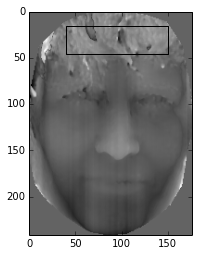
\includegraphics[width=\columnwidth]{images/face1}
        \subcaption{}
        \label{subfig:robust-face1}
    \end{subfigure}
    \hfill
    \begin{subfigure}{0.45\columnwidth}
        \centering
        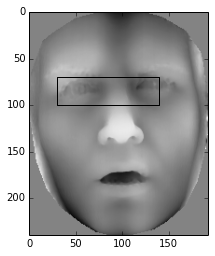
\includegraphics[width=\columnwidth]{images/face2}
        \subcaption{}
        \label{subfig:robust-face2}
    \end{subfigure}
    \caption{The images used to produce the results in Figure~\ref{fig:robust-properties}.}
    \label{fig:robust-faces}
\end{figure}
%%%%%%%%%%%%%%%%%%%%%%%%%%%%%%%%%%%%%%%%%%%%%%%%%%%%%%%%